% !TeX root = ../diss.tex

\chapter{Implementation}

\section{C implementation}
\label{sec:C_impl}

\subsection{Initial implementation}
\label{sec:Initial_C_impl}

First, I implemented Smith-Waterman’s algorithm in single-threaded C code.
I started with a simple implementation that stored the entire grid in a 2D array and calculated grid cells sequentially, which involved rewriting the definitions of the Smith-Waterman algorithm in C.
An excerpt (where \lstinline{decideCellSW} is similar to a \lstinline{max} function but also returns a pointer) is \cref{lst:c_sw}.

\begin{lstlisting}[language=C,float,basicstyle=\linespread{0.9}\ttfamily\footnotesize, label={lst:c_sw},captionpos=b,caption={Excerpt from C implementation of Smith-Waterman algorithm}]
for (unsigned long i = 0; i < len1; i++) {
    for (unsigned long j = 0; j < len2; j++) {
        decisions[i+1][j+1] = decideCellSW(
                decisions[i][j].score + match(seq1[i], seq2[j]),
                decisions[i][j+1].score + GAP_PENALTY,
                decisions[i+1][j].score + GAP_PENALTY
        );
        if (decisions[i+1][j+1].score >= bestCell->score) {
            bestCell->score = decisions[i+1][j+1].score;
            bestCell->i = i+1;
            bestCell->j = j+1;
        }
    }
}
\end{lstlisting}
This simple implementation did not perform very well, especially with long strings.
It is single-threaded, and the grid takes $O(NM)$ space for sequences of lengths $N$ and $M$.
Space was a major issue; working with the large grid in RAM was costly.
The number of alignments that could be run in parallel was limited due to memory constraints.
This is quantified in \cref{sec:C_impls_eval}.
However, this quadratic space implementation was used as a component of the linear space variant, and it also was the basis of my correctness testing (\cref{sec:Correctness_eval}).

\subsubsection{Back-tracing}
\label{sec:Initial_C_back_tracing}
In this implementation, nearly all of the time was spent filling out the of the grid (\cref{sec:C_occupancy}).
After this, an alignment was produced using a process called back-tracing (\cref{sec:SW_Back_tracing}). Stored with each grid cell is a ``pointer'' which locates the previous cell in the best alignment ending with that cell.

Using these pointers, starting at the best cell in the grid, a pair of aligned sequences is built up from back to front by following the pointers upwards and leftwards to a cell with a $Nil$ pointer.
This takes as many steps as there is symbols in the alignment, and an upper bound on this is $N+M$ steps for sequences of lengths $N$ and $M$.

\subsubsection{Linear space implementation}
\label{sec:Initial_C_Linear}
This implementation was a direct implementation of the algorithm described in \cref{sec:SW_Linear_Prep}.
It was slower than the quadratic space implementation, which was unsurprising because twice as much arithmetic was involved (\cref{sec:SW_Linear_Complexity}).
However, the implementation only took $50\%$ longer due to decreased memory usage and associated memory overheads (\cref{sec:C_impls_eval}).
Due to decreased memory usage there were not issues with performing multiple alignments at the same time, and the structure of the algorithm was amenable to parallelisation.

\subsection{Multi-threaded implementation}
\label{sec:Multi_threaded_C_impl}
This linear-space algorithm (\cref{sec:SW_Linear_Prep}) was simple to parallelise, because each grid could be processed in parallel.
Memory consistency is trivial to maintain because no data is shared between running threads; threads just join after processing their grid segment.
However, given infinite threads there is still a finite speedup, because the number of different segments of the grid available for evaluation is limited.
This limit increases as the algorithm progresses.
At the start, there are two grid segments (each taking half of the whole grid) being evaluated to find their middle columns.
If the optimal alignment crosses the middle column, the algorithm is applied recursively between the chosen cell in the middle column, and the top-left or bottom-right of the rest of the grid.
This has four sub-grids (a forwards and backwards one on each side of the middle column), covering a total area of half of the grid. Assuming infinite threads, this generalises to:
$$\text{Cells evaluated } = \frac{1}{2} \times NM + \frac{1}{4} \times \frac{NM}{2} + \frac{1}{8} \times \frac{NM}{4} + \cdots \leq \frac{1}{2} \times NM \sum_{i=0}^\infty 2^{-2i} = \frac{2NM}{3}$$

This limit was not reached in practice (\cref{sec:C_impls_eval}) but it is useful to consider.
To improve on this limit, there would need multiple threads working on each segment of the grid.
A major concern with this is synchronising threads such that they only evaluate cells when the cells they depend on have been evaluated by a different thread.
This could yield poor performance due to threads waiting on each other, and for this reason I did not prioritise implementing this approach, and I did not have time to do so.
GPUs and FPGAs are attractive platforms for solving this problem because they make it very simple to schedule threads relative to one another.

\subsubsection{Synchronisation and scheduling of work}
\label{sec:Sync_and_scheduling_of_multi-threaded_C}
I used the Native POSIX Thread Library, part of the GNU C Library, to implement this multithreaded solution.
The scheduling of threads is handled by the library and the host operating system.
By assigning the work to fill out the two halves of a grid to two different threads, and also the two recursive calls of the linear space solver to different threads, the linear space algorithm is straightforward to parallelise.
This can be seen in \cref{fig:Linear_Space_Structure}, where the numbered blocks can each be evaluated by a different thread.

My implementation was slightly more complex, allowing me to investigate how the number of available CPU cores changed the throughput of my implementation.
The results of this are presented in \cref{sec:C_params_eval}.
This was achieved using a counting semaphore to represent the number of concurrent threads performing arithmetic.
This semaphore guards the regions that were evaluating grid cells, which corresponds to the \cref{lst:pseudo_sw,lst:pseudo_sw_col}.
Threads about to enter these regions wait on the semaphore, and signal the semaphore when they leave those regions.
The effect of different numbers of working threads could be evaluated by changing the size of the semaphore.
The highest throughput on my 6-core SMT CPU was achieved using 12 threads (\cref{sec:C_params_eval}).

\subsection{Sequence similarity functions and scoring gaps}
\label{sec:Scoring_in_C_impl}
The two forms of sequence similarity function discussed in \cref{sec:SW_similarity_functions} were implemented, and the performance was evaluated later (\cref{sec:C_scoring_eval}).

Both the linear and affine gap scoring mechanisms were implemented.
The linear space implementation needed to account for horizontal gaps being opened on one side of the middle column but continued through to the other side.
This can be solved by adding the middle columns coming for both the the gap matrix $P_{i,j}$ and the score matrix $H_{i,j}$.
These decisions also need to be propagated into the sub-problems as well.
This was the approach taken by Myers and Miller \cite{MyersMiller} in their adaption of Hirschberg’s algorithm \cite{Hirschberg} to local alignment.

\section{CUDA implementation}
\label{sec:CUDA_impl}
My implementation in CUDA took a similar approach to the C implementation but using a streaming multiprocessor to evaluate many grid cells in parallel on the same device.
The SIMT (single-instruction, multiple-thread) architecture makes it is easier to synchronise work between multiple threads running the same instructions.
In CUDA there are two broad categories of parallelism: parallelism between threads (parallelism inside a multiprocessor), and parallelism between blocks (parallelism between multiprocessors).
Each of these were utilised in my implementation.

\subsection{Parallelism between threads}
\label{sec:Thread_Parallelism_in_CUDA}
Multiple threads run inside of a block simultaneously, scheduled in warps of $32$ threads, with shared memory and barrier synchronisation to allow for cooperation between threads in different warps.
I built up a diagonal front of threads, so that threads only depend on results that other threads have already computed.
This is similar to the approach taken by Ling et al. \cite{Ling_GPU}, however in their approach they exploit parallelism between blocks by running multiple alignments at the same time, whereas I chose to use multiple blocks in a single alignment.
Under my design multiple different alignments can also be running in parallel, but large and difficult alignments can exploit more than one streaming multiprocessor.

Threads on the anti-diagonal to the grid have no data dependencies and can be executed in parallel.
This is the basis for much of the parallelisation in the GPU and FPGA implementations.
This can be seen in \cref{fig:Diagonalised_Grid}, where dark grey cells have already been computed, and light grey cells can all be computed in parallel.
Dependencies between cells are shown as red arrows.

\begin{figure}
  \centering
  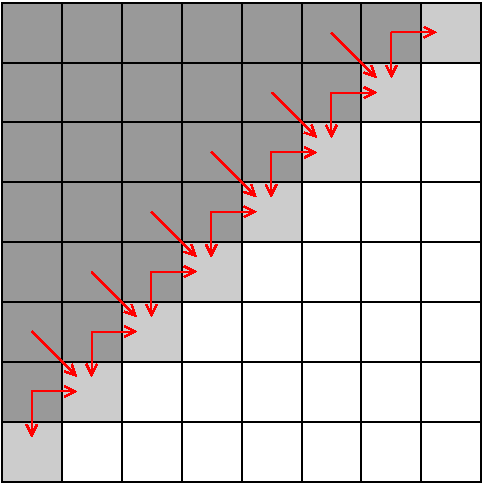
\includegraphics[width=\textwidth/2]{figs/diagonalised_grid.pdf}
  \caption{An anti-diagonal of data dependencies in Smith-Waterman’s algorithm}
  \label{fig:Diagonalised_Grid}
\end{figure}

The general approach is to assign each column to a thread and stagger the threads so that if thread $t$ is working on row $r$, then thread $t+1$ is working on row $r+1$.
Threads are then synchronised using a barrier so that only one anti-diagonal is being computed at a time.
With an unlimited number of threads, the time spent calculating the grid changes from being quadratic to linear in sequence length, taking $N + M - 1$ steps because there are that many anti-diagonals in a grid of dimensions $N\times M$.

In reality, there is a limit to the number of threads allowed in a block in CUDA ($1024$ threads), and only $32$ threads of a given block can be executing at once.
Therefore, every column cannot be assigned its own exclusive thread.
My first approach was to have a single block of threads generate the entire grid, by generating blocks of columns at a time, where each individual column had its own thread and upon reaching the end of the columns, new blocks of columns were generated.
However, when profiling my program using NVProf, it suggested that a way to improve performance might be to spread my work out over multiple thread blocks, which would spread the work over multiple streaming multiprocessors.
This had a noticeable performance improvement (\cref{sec:CUDA_single_multi_block_eval}).

\subsection{Parallelism between blocks}
\label{sec:Block_Parallelism_in_CUDA}

The opportunity for parallelism described in \cref{sec:Thread_Parallelism_in_CUDA} exists between blocks of threads, as well as threads themselves.
Although squares in \cref{fig:Diagonalised_Grid} represent threads, it also is an accurate representation when squares represent blocks as well.
This is the basis of my implementation for generating the grid using multiple blocks at once.

However, a different approach needs to be taken for communications between different anti-diagonals.
It is possible to impose an ordering of execution between threads in a block, but it is not possible to impose an ordering between blocks of a kernel grid.
There is no guarantee on the order in which blocks may be executed, there is a limit to the number of blocks that can be resident on the device, and blocks cannot leave the device until they have finished executing.
Therefore, attempting to impose an ordering by building up concurrency primitives from global memory may lead to deadlock.

Therefore, the kernel needs to be broken up into multiple smaller kernels, where blocks have no dependencies on one another.
This is done using the approach outlined above on the block-scale, where a kernel is made up of an anti-diagonal of blocks, and the number of blocks depends on the size of the grid and which anti-diagonal is being computed.
Each block writes out its right and bottom edges to global memory on the device, ready for the next block from the next kernel to consume.
All the data remains on the device so there is relatively little overhead in making many blocks for relatively short periods of time.

\subsection{Memory types}
\label{sec:Memory_in_CUDA}

The grid of scores and pointers is stored in the global memory, which is the GDDR5 VRAM used by the GPU.
There is $\SI{4}{\gibi\byte}$ of this in my laptop and it has much higher bandwidth than the DDR4 main memory in the laptop.
GPUs are designed to hide memory access latency for this memory by context switching between many different threads, so it is a good fit for this algorithm with many loads and stores.

Alternatively, shared memory (on the die of the GPU) could have been used but this is too small with only $\SI{1152}{\kibi\byte}$ available.
A block of $1024$ threads has access to only $\SI{48}{\kibi\byte}$, with room for a $78\times78$ cell grid.
With a capacity of $\SI{4}{\gibi\byte}$, the GDDR5 VRAM, was the best choice for storing the grid.

\subsection{Back-tracing}
\label{sec:Back_tracing_in_CUDA}

Back-tracing is performed on the GPU.
Even though it is a sequential process that only uses one thread of a $32$-thread multiprocessor, it is significantly quicker than it would be to copy the entire grid out of VRAM into RAM, and have the CPU run the back-tracing.
To back-trace on the CPU, too much time would be wasted copying over unwanted data: only $N+M$ grid cells could be needed out of the $N\times M$ cell grid, and finding which are needed is the process of back-tracing.

\subsection{Linear space improvements}
\label{sec:Linear_space_CUDA}

For similar reasons to the C implementation, there are performance limitations when using this quadratic space algorithm.
For large sequences memory will simply run out; a $\SI{23710}{} \times \SI{23170}{}$ grid is the largest grid that will fit in the $\SI{4}{\giga\byte}$ VRAM.
Fortunately, the linear space algorithm (\cref{sec:SW_Linear_Prep}) can also be implemented in CUDA using the same techniques discussed in \cref{sec:Thread_Parallelism_in_CUDA,sec:Block_Parallelism_in_CUDA,sec:Memory_in_CUDA,sec:Back_tracing_in_CUDA}.

Using this approach the problem is divided in half repeatedly; calculating the scores for the middle column using linear space to decide where to divide.
The control logic was implemented on the host device (the CPU), but the evaluation of grid cells and back-tracing of alignments was done on the GPU.
This was a sensible choice because most of the control flow decisions are sequential which would poorly utilise 32-thread multiprocessor on the GPU.
Moreover, the CPU achieves a much higher clock frequency and sequential throughput than the GPU.

Calculating a half-grid segment requires multiple kernel invocations for each segment, so the control logic was also multi-threaded where each segment had its own thread.
This was facilitated by CUDA Streams, which are similar to OS processes or threads.
When evaluating a grid, all of the blocks on the current anti-diagonal need to have finished before the next anti-diagonal can be processed, and the CPU can only synchronise with the GPU when either the entire GPU finishes all available work, or when all work in a stream has finished.
With each thread of C code assigned its own CUDA stream, the thread can synchronise with the work it has sent to the GPU whilst leaving other streams (and therefore threads) to utilise the GPU at the same time.
The first few and last few anti-diagonals of a grid will have fewer blocks of work than streaming multiprocessors available, so utilisation of these multiprocessors can be increased by using multiple concurrent streams of work, working on different parts of the alignment.

Using this implementation to compare multiple sequences at once is trivial, simply a new thread and stream is created for each alignment, and all subsequent new threads and streams required will be created by the alignment program.
All scheduling is done by the operating system and GPU hardware, which should lead to maximum resource utilisation provided there is the work to consume it.

\subsection{Sequence similarity functions and scoring gaps}
\label{sec:Scoring_in_CUDA_impl}

The same approach to sequence similarity functions and scoring gaps taken for the C implementation (\cref{sec:Scoring_in_C_impl}) was also used for the CUDA implementation.
The more complex scoring mechanisms such as similarity matrices and affine gaps had a performance penalty which is discussed in \cref{sec:CUDA_scoring_eval}.

\section{SystemVerilog implementation for FPGA}
\label{sec:SV_impl}

My SystemVerilog implementation was a systolic array.
This is an approach which has been used before \cite{FPGA_Impl}, and is sensible given the structure of the problem.
A systolic array is a sequence of processing elements (PEs), where each element produces signals to be used by the next element in the array.
This can be used to encode the horizontal data dependencies between grid cells in SystemVerilog, which in turn will lead to the data dependencies being represented in routing hardware.
The vertical data dependencies can be encoded into each PE.

The approach is simplest to explain using small fixed-length sequences, but it can be generalised to arbitrary length sequences.
Each PE calculates the scores and pointers for a different column in the grid, where the PE can evaluate a cell every cycle.
The value above the current cell was calculated by the same PE and is remembered by that PE.
The values to the left and diagonal are calculated by the previous PE, and this passed from one PE to the next.

The cells being evaluated in the array follow an anti-diagonal of the grid.
This is achieved by passing `enable' signals down the array to form a shift register, with the first PEs to be enabled also are the first to be disabled because they reach the bottom of the grid first.
This architecture is called a systolic array, with data pumping in and out of the array like a heart pumping blood \cite{SystolicArrays}.

Each PE only needs to store one sequence symbol for the column, because this remains constant, and the symbol relating to the row can propagate through the array.
Each PE also keeps a running maximum score and position, and sends this down the array.
The last element will output the maximum score and position for the entire grid, which is where the back-tracer will start from.

The scores are only required for a brief period; they are only used in the evaluation of three cells. Instead of storing this in some external data structure, this can be embedded in the registers of each processing element and stored within the systolic array.
An array of pointers still needs to be maintained for back-tracing, and this became a limiting factor of my design.

To modify this design to work with sequences of variable length, a first-in first-out (FIFO) queue is required to buffer a column of scores.
Each column is still processed by one PE, but for an array of length $n$ the PE at index $i$ will process columns $kn+i < N$ for integers $k$ and sequence length $N$.
The PE at the end of the array writes its scores out to the FIFO, and when the first PE reads these scores from the FIFO to produce the next block of columns.
This approach will work for sequences of any length, but in practice is limited by memory capacity for storing this FIFO and grid of pointers.
\Cref{fig:Medium_Systolic_Array} is an overview of the systolic array, and \cref{fig:PE_Cell} shows the structure of a processing element.

\begin{figure}
    \centering
    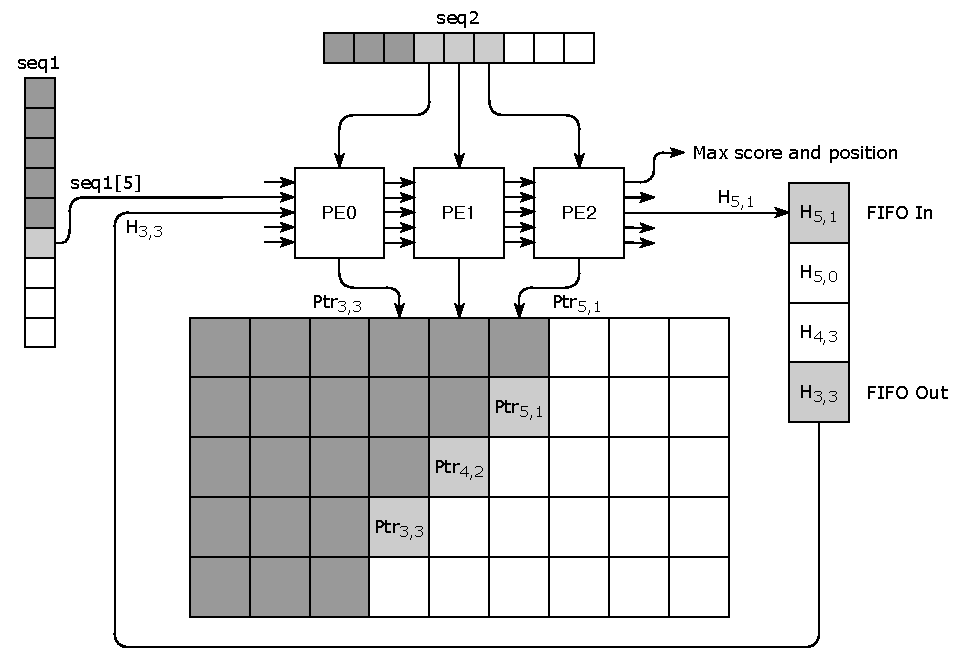
\includegraphics[width=0.9\textwidth]{figs/med_systolic_array.pdf}
    \caption{An overview of the systolic array}
    \label{fig:Medium_Systolic_Array}
\end{figure}

\begin{figure}
    \centering
    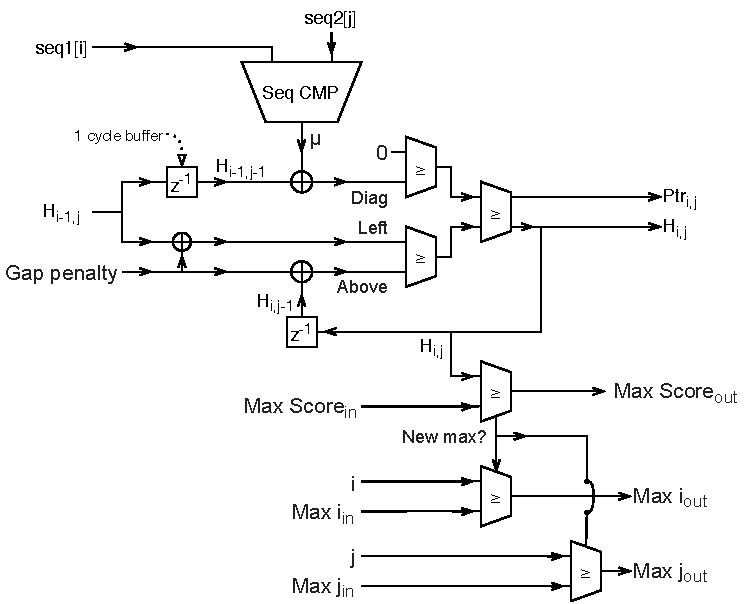
\includegraphics[width=0.75\textwidth]{figs/pe_cell.pdf}
    \caption{The structure of a single processing element in the systolic array}
    \label{fig:PE_Cell}
\end{figure}

\subsection{Device memory limitations}
\label{sec:Memory_in_SV}

The limiting factor is needing to store this array of pointers.
Each pointer can be one of four values, so $\SI{2}{\bits}$ per pointer was required.
For two sequences of lengths $N$ and $M$, $N\times M$ such pointers are required.
In each cycle each PE could be writing out a pointer, and this bandwidth requirement also influenced the choice of what type of memory to use.

There are several different types of memory on the development board I used, with different characteristics (\cref{tab:FPGA_Memories}).
Bandwidth limitations to the highest capacity memory devices (the $\SI{64}{\mebi\byte}$ SDRAM for the FPGA, and the $\SI{1}{\gibi\byte}$ SDRAM for the HPS) would have limited the size of the systolic array to $8$ or $32$ PEs respectively, due to their 16-bit and 64-bit buses.
I instead chose to use the M10K embedded memory blocks, which is the largest collection of memory that does not have these bandwidth limitations.

Instead, the design was limited by the number of M10K blocks available.
There are $397$ M10K blocks on the board I was using, giving $\SI{3970}{\kibi\bit}$ of total memory; approximately 2 million possible pointers or a $1425\times1425$ grid.
In practice, $5$ M10K blocks were used in the interface between the HPS and FPGA, and the FIFO needed to be stored.
The FIFO is either $N$ or $M$ $\SI{16}{\bit}$ twos-complement integers long.
On top of this, each processing element needs exclusive access to the memory blocks for each part of the grid, if each processing element is to write every cycle.
Sharing blocks between PEs would have added complexity, and likely caused delays and hazards in the design.

With these constraints in mind, I chose the maximum sequence lengths of this implementation to be $1024\times1536$ symbols.
This grid can fit in $384$ M10K blocks, using $96.7\%$ of the blocks available.
The FIFO is $1024$ words long, and fits in $2$ M10Ks.
The systolic array had $48$ PEs, with each PE writing to $8$ M10K blocks of pointer grid.
Due to the factor of $3$ in $1536$, the length of the systolic array needs to be a multiple of $3$ to allow each M10K to be assigned to exactly one PE.
Due to this addressing constraint, the next largest systolic array that would work under this arrangement would have $96$ elements each with $4$ M10Ks.
However, the $48$ PE array requires $62\%$ of the logic elements when aligning DNA, and $93\%$ when aligning proteins (\cref{sec:FPGA_utilisation}).
In both cases, doubling the number of PEs was not possible without a larger FPGA.

With a more modern FPGA, such as a similarly priced Cyclone 10 FPGA to the Cyclone V when that was first sold, would have nearly double the logic elements and quadruple the amount of embedded memory \cite{Cyclone10}.
My design would likely be able to be instantiated as a $96$ PE array, and could align sequences of lengths $2048$ and $3072$, probably at a higher clock speed as well.

\subsection{Back-tracing}
\label{sec:Back_tracing_in_SV}

Back-tracing involves starting at the best cell found by the systolic array, and following the pointers through the grid.
A minor challenge was that it takes a cycle between requesting an address from a M10K block and getting the data out.
It is possible to pipeline requests, where the next address is requested whilst the previous address is being read out, but this would have been complex to implement.
This meant that back-tracing takes two cycles per aligned symbol, with an upper bound on the number of cycles spent back-tracing being $2\times(N+M)$.

I chose not to pipeline this because back-tracing only takes a small amount of the overall execution time.
When aligning sequences of lengths of $1024$ and $1536$, only $13\%$ of the time is spent back-tracing (\cref{sec:Processing_time_on_FPGA}).
Using Amdahl’s law, if I could improve back-tracing to only take one cycle per symbol, the expected speedup is $1.07$ times; it would not have a significant impact overall processing time.
$$Speedup = \frac{1}{87\% + \frac{1}{2}\times 13\%} = 1.07 $$

\subsection{Processing time}
\label{sec:Processing_time_on_FPGA}
It is possible to derive exactly the amount of time it will take to align two sequences when working with FPGAs with constant clock frequencies.
For the design described above, with $48$ PEs in the systolic array, and sequences of lengths $N$ and $M$, the runtime is as follows.

For a 48-column section of the grid, it takes $48$ cycles for the last column to begin being evaluated, and then $N$ cycles to reach the bottom of that last column, requiring $N+48$ cycles in all.
One additional cycle is required, to find the diagonal score for the first column.
In conclusion, each 48-column section of the grid takes $N+49$ cycles to evaluate.

The number of 48-column segments in the grid is $\left \lceil \frac{M}{48} \right \rceil$.
Even when processing the last segment, which may have fewer than $48$ columns to consider, the device must wait $N+49$ cycles because the best score and location needs to propagate to the last PE, from which it is read by the back-tracing logic.
Combining this, the number of cycles required to produce the grid is ${(N+49) \times \left \lceil \frac{M}{48} \right \rceil}$

As discussed in the \cref{sec:Back_tracing_in_SV}, the amount of time required by the back-tracing logic is bounded by $2\times(N+M)$, so the number of cycles required for an alignment is:
$$\text{Runtime} = (N+49) \times \left \lceil \frac{M}{48} \right \rceil + 2 \times (N+M)$$

This expression is $O(NM)$.
Evaluating this expression with the maximum sequence lengths of $1024$ and $1536$ from previous section:
$$\text{Runtime} = (1024+49) \times \left \lceil \frac{1536}{48} \right \rceil + 2 \times (1024+1536) = \SI{39456}{\cycles}$$
Where $5120$ of the $\SI{39456}{}$ cycles ($13\%$) are spent back-tracing and the rest on filling the grid.
For the design which aligned DNA sequences I was able to clock my logic at $\SI{79}{\mega\hertz}$ using a PLL, so this pair of DNA sequences requires $\SI{499.4}{\micro\s}$ to execute.
Due to the additional complexity when aligning proteins my design could only run at $\SI{60}{\mega\hertz}$, so this pair of protein sequences requires $\SI{657.6}{\micro\s}$ to execute.
These limitations are discussed in \cref{sec:SV_Fmax}.

\subsection{Sequence similarity functions and scoring gaps}
\label{sec:Scoring_in_SV_impl}

Sequence similarity functions and gap penalty values were compiled into the hardware.
This reduces the flexibility of a compiled design, but this was sufficient for the testing I was doing.
For aligning nucleotides, I used a constant sequence similarity function and for aligning proteins I used the BLOSUM50 scoring matrix.
Representing one of four nucleotides takes $\SI{2}{\bits}$ but representing one of $22$ amino acids takes $\SI{5}{\bits}$.
This increased representational cost, alongside the quadratically scaled lookup table to align symbols, leads to the increased logic utilisation for the protein aligning circuit and also a lower maximum clock speed of that design (\cref{sec:FPGA_utilisation}).

I did not have the time to implement an affine gap scoring mechanism (\cref{sec:SW_gaps}) in my FPGA implementation, but the entire FPGA implementation was a project extension.
I expect it would not have had a major performance penalty.
The number of scores that need to be stored will triple (to cover three grids instead of one), but the systolic array only stores a small number of these scores to begin with.
The number of comparisons inside PEs would increase by two per cycle (one for each gap matrix), and only increase the comparison tree depth by one level.

\section{Repository overview}
\label{sec:Repo_overview}

My source code repository is divided into three sections (\lstinline{cpu_code}, \lstinline{gpu_code}, \lstinline{fpga_code}) which reflect the three major implementations of my project.
All code in it has been written from scratch, apart from the FPGA-HPS interfaces (\lstinline{fpga_code/systemverilog/*_avalon.sv}, and the contents of \lstinline{fpga_code/c_interface/}) which are based on code from my supervisor Peter Rugg, as discussed in \cref{sec:Starting_Point}.
A detailed overview can be found in \cref{fig:Repo_tree}.

% !TeX root = ./diss.tex

\DTsetlength{0.2em}{1em}{0.2em}{1pt}{4pt}
\begin{figure}[H]
\dirtree{%
    .1 /.
    .2 cpu\_code\DTcomment{C implementation}.
        .3 correctness\_tester.c \DTcomment{Basis for correctness testing across implementations}.
        .3 helpers.c \DTcomment{Utility functions}.
        .3 main.c \DTcomment{Entry point; rudimentary command line interface}.
        .3 nw.c \DTcomment{Initial global alignment implementation}.
        .3 sw.c \DTcomment{Local alignment implementation, quadratic and linear space}.
        .3 swParallel.c \DTcomment{Multi-threaded local alignment implementation}.
        .3 swGotoh.c \DTcomment{Affine gap implementation, quadratic and linear space}.
        .3 swGotohParallel.c \DTcomment{Multi-threaded affine gap alignment implementation}.
    .2 gpu\_code\DTcomment{CUDA implementation}.
        .3 helpers.cu \DTcomment{Utility functions}.
        .3 main.cu \DTcomment{Entry point; rudimentary command line interface}.
        .3 sw.cu  \DTcomment{Local alignment implementation, quadratic and linear space}.
        .3 swSingleBlock.cu \DTcomment{Quadratic space local alignment, without block-parallelism}.
        .3 swGotoh.cu \DTcomment{Affine gap implementation}.
    .2 fpga\_code\DTcomment{FPGA implementation}.
        .3 c\_interface \DTcomment{C Interface for ARM HPS}.
            .4 sequence\_reader.c \DTcomment{Reading sequences from files}.
            .4 start.c \DTcomment{Interface with FPGA}.
        .3 systemverilog \DTcomment{SystemVerilog implementation}.
            .4 datatypesPkg.sv \DTcomment{Types of signals used}.
            .4 macro.vh \DTcomment{Implementation-wide macros to change types of sequences}.
            .4 pe\_bram.v \DTcomment{BRAM for grid of pointers}.
            .4 fifo\_16b\_1024w.v \DTcomment{BRAM FIFO for storing previous column of scores}.
            .4 backtrace.sv \DTcomment{Backtracing through a grid of registers}.
            .4 backtrace\_with\_ram.sv \DTcomment{Backtracing through a grid in M10K BRAM}.
            .4 pe.sv \DTcomment{Single processing element where pointer grid is registers}.
            .4 pe\_with\_ram.sv \DTcomment{Single processing element where pointer grid is BRAM}.
            .4 short\_solver.sv \DTcomment{Systolic array for sequences the length of the array}.
            .4 short\_solver\_avalon.sv \DTcomment{Avalon FPGA-HPS interface for \lstinline{short_solver}}.
            .4 med\_solver.sv \DTcomment{Systolic array for sequences of lengths $1024 \times 1536$}.
            .4 med\_solver\_with\_ram.sv \DTcomment{\lstinline{med_solver} but using BRAM for pointer grid}.
            .4 med\_solver\_with\_ram\_avalon.sv \DTcomment{Main Avalon FPGA-HPS interface}.
            .4 tb\_blosum.sv \DTcomment{Various testbenches (\lstinline{tb_*})}.
            .4 tb\_med\_solver.sv .
            .4 tb\_med\_solver\_with\_ram.sv .
            .4 tb\_pe.sv .
            .4 tb\_short\_seq.sv .
            .4 tb\_short\_solver.sv .
        .3 quartus \DTcomment{Configuration files from my Quartus Lite project}.
}
\caption{Header files (of extensions \lstinline{.h} and \lstinline{.cuh}) have been omitted from for brevity, and always correspond to a code file. Makefiles have also been omitted.}
\label{fig:Repo_tree}
\end{figure}

